% Drawing 80/03-6 -- folder 80, batch 03, archive page 56 (PDF page 57).
% Transcription: dessin à l'encre : dix droites, deux verticales épaisses, deux horizontales et six obliques, avec cinq sommets quadruples marqués d'un point noir (les quatre coins du carré central et un point à l'intérieur) ; chaque région porte le nombre de ses côtés, $3$, $4$ ou $5$ (une seule région $5$, en bas au centre), les régions du haut « id »
% Kind: arrangement of ten lines with five quadruple points. Method 2 (schematic redraw from the facsimile). Status: ok.
% Notes: Ink. Ten lines: the two verticals and two horizontals of the central square, its two diagonals, and four lines each through one corner and the inner point; every line is drawn through its marked points, so that four lines meet exactly at each of the five dots. Which oblique passes through which dot was read on a 600 dpi crop and agrees with his count: ten lines with five quadruple points and fifteen simple crossings give 31 regions. Region labels 3, 4, 5 and « id » (the upper regions, the same as the lower ones across infinity) as on the page. Left out: a small overwritten digit beside the lower left dot; the heavy 3 at the left is written over an earlier digit. The transcription's note does not count the lines. Redrawn 2026-11-12 (issue 128): to check again.
% Coordinates: 1 unit = 1 mm = 1/100 of the crop width (bbox in page fractions: [0.1, 0.075, 0.83, 0.52]).
% Redrawn by Claude (claude-fable-5-2), issue #128, 2026-11-12; not checked by a human; not compiled (no TeX in the session).
% Rights: reproduces part of the work -- behind RENDER_TRANSCRIPTS, never published by itself.
\documentclass[tikz,border=3pt]{standalone}
\usepackage{amsmath,amssymb}
\usetikzlibrary{patterns,arrows.meta}
\tikzset{pencil/.style={black!45}, struck/.style={black!35}, mpt/.style={circle,draw,inner sep=1.3pt}, pt/.style={circle,fill,inner sep=0.9pt}, opt/.style={circle,draw,fill=white,inner sep=1.1pt}}
\begin{document}
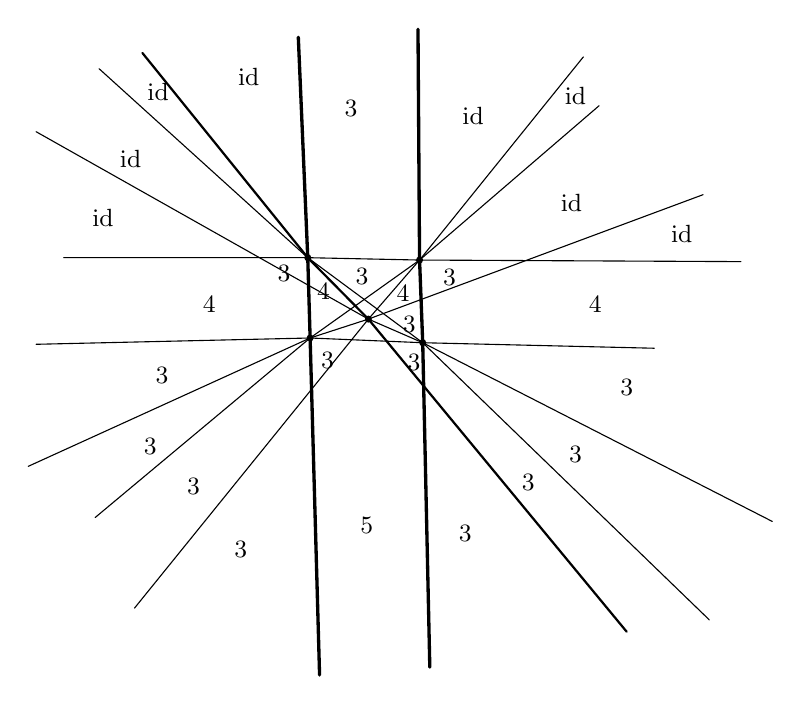
\begin{tikzpicture}[x=1mm,y=1mm,line cap=round,line join=round,font=\scriptsize]
\draw[very thick] (37.3,-3) -- (38.5,-31) -- (38.8,-41.2) -- (40,-84);
\draw[very thick] (52.5,-2) -- (52.7,-31.3) -- (53.1,-41.8) -- (54,-83);
\draw (7.5,-31) -- (38.5,-31) -- (52.7,-31.3) -- (93.5,-31.5);
\draw (4,-42) -- (38.8,-41.2) -- (53.1,-41.8) -- (82.5,-42.5);
\draw (12,-7) -- (38.5,-31) -- (53.1,-41.8) -- (89.5,-77);
\draw (75.5,-11.7) -- (52.7,-31.3) -- (38.8,-41.2) -- (11.5,-64);
\draw[thick] (17.5,-5) -- (38.5,-31) -- (46.2,-38.8) -- (79,-78.5);
\draw (73.5,-5.5) -- (52.7,-31.3) -- (46.2,-38.8) -- (16.5,-75.5);
\draw (3,-57.5) -- (38.8,-41.2) -- (46.2,-38.8) -- (88.7,-23);
\draw (4,-15) -- (46.2,-38.8) -- (53.1,-41.8) -- (97.5,-64.5);
\node[pt] at (38.5,-31) {};
\node[pt] at (52.7,-31.3) {};
\node[pt] at (38.8,-41.2) {};
\node[pt] at (53.1,-41.8) {};
\node[pt] at (46.2,-38.8) {};
\node[inner sep=1pt] at (31,-8) {\small id};
\node[inner sep=1pt] at (19.5,-10) {\small id};
\node[inner sep=1pt] at (16,-18.5) {\small id};
\node[inner sep=1pt] at (12.5,-26) {\small id};
\node[inner sep=1pt] at (59.5,-13) {\small id};
\node[inner sep=1pt] at (72.5,-10.5) {\small id};
\node[inner sep=1pt] at (72,-24) {\small id};
\node[inner sep=1pt] at (86,-28) {\small id};
\node[inner sep=1pt] at (44,-12) {\small $3$};
\node[inner sep=1pt] at (35.5,-33) {\small $3$};
\node[inner sep=1pt] at (45.4,-33.4) {\small $3$};
\node[inner sep=1pt] at (56.5,-33.5) {\small $3$};
\node[inner sep=1pt] at (51.4,-39.5) {\small $3$};
\node[inner sep=1pt] at (41,-44) {\small $3$};
\node[inner sep=1pt] at (52,-44.3) {\small $3$};
\node[inner sep=1pt] at (20,-46) {\small $3$};
\node[inner sep=1pt] at (79,-47.5) {\small $3$};
\node[inner sep=1pt] at (18.5,-55) {\small $3$};
\node[inner sep=1pt] at (24,-60) {\small $3$};
\node[inner sep=1pt] at (30,-68) {\small $3$};
\node[inner sep=1pt] at (58.5,-66) {\small $3$};
\node[inner sep=1pt] at (66.5,-59.5) {\small $3$};
\node[inner sep=1pt] at (72.5,-56) {\small $3$};
\node[inner sep=1pt] at (40.5,-35.3) {\small $4$};
\node[inner sep=1pt] at (50.6,-35.6) {\small $4$};
\node[inner sep=1pt] at (26,-37) {\small $4$};
\node[inner sep=1pt] at (75,-37) {\small $4$};
\node[inner sep=1pt] at (46,-65) {\small $5$};
\end{tikzpicture}
\end{document}
